
\documentclass[a4paper]{article}
\usepackage[a4paper,margin=1in]{geometry}
\usepackage{authblk}
\usepackage{booktabs}
\usepackage[shortlabels]{enumitem}
\usepackage[table,xcdraw]{xcolor}
\usepackage{graphicx}
\setlength\headheight{15pt}
\colorlet{headbgcolor}{orange}
\usepackage[markcase=noupper]{scrlayer-scrpage}
\usepackage[english]{babel}
\usepackage{hyperref}
\usepackage{adjustbox}
\usepackage{float}
\usepackage{blindtext}
\usepackage{multirow}
\usepackage{dcolumn}% Align table columns on decimal point
\usepackage{bm}% bold math
\usepackage{hyperref}% add hypertext capabilities
\usepackage[english]{babel}
\usepackage{caption}
\usepackage{subcaption}
\usepackage{siunitx}
\usepackage{amsmath}
\usepackage{tabularx}
\usepackage[super]{nth}
\clearpairofpagestyles
%\automark[chapter]{chapter}
%\renewcommand\chaptermarkformat{\chaptername\ \thechapter:\enskip}
\setlength{\parskip}{1em}
\renewcommand{\baselinestretch}{1.2}

\title{\textbf{Title}}
\author{Author}
\date{Date}

\begin{document}

\maketitle



\section*{Objective}

\begin{enumerate}
\item Objectives
\end{enumerate}



\section*{Apparatus}



\begin{itemize}
\item Apparatus
\end{itemize}


\section*{Theory}

Theory here

\section*{Observations}

\begin{table}[htb]
    \centering
    \begin{tabular}{@{}cccccc@{}}
        \toprule
         & Temperature (in $^oC$) & $V_R$ & $V_C$ & DC Capacitance (in nF) & AC Capacitance (nF) \\
        \midrule
         & 102 & 4.21 & 1.59 & 1.08 & 0.192 \\
         & 101 & 4.25 & 1.6 & 1.07 & 0.192 \\
         & 100 & 4.2 & 1.57 & 1.05 & 0.194 \\
         & 99 & 4.15 & 1.56 & 1.03 & 0.192 \\
         & 97 & 4.2 & 1.54 & 1.00 & 0.197 \\
         & 95 & 4.17 & 1.54 & 0.95 & 0.196 \\
         & 93 & 4.15 & 1.51 & 0.92 & 0.199 \\
         & 91 & 4.07 & 1.5 & 0.88 & 0.196 \\
         & 90 & 4.07 & 1.49 & 0.86 & 0.198 \\
         & 85 & 4.04 & 1.45 & 0.8 & 0.202 \\
         & 75 & 3.58 & 1.43 & 0.73 & 0.181 \\
         & 70 & 3.96 & 2.12 & 0.7 & 0.135 \\
        \bottomrule
    \end{tabular}
\end{table}
\begin{table}[htb]
    \centering
    \begin{tabular}{@{}cccccccc@{}}
        \toprule
         &  & Temperature (in $^oC$) & $V_R$ & $V_C$ & DC Capacitance (in nF) & AC Capacitance (nF) &  \\
        \midrule
         &  & 21.3 & 3.92 & 1.95 &  & 0.145 &  \\
         &  & 50 & 3.95 & 1.95 & 0.63 & 0.147 &  \\
         &  & 55 & 3.95 & 1.94 & 0.65 & 0.147 &  \\
         &  & 60 & 3.96 & 1.93 & 0.64 & 0.148 &  \\
         &  & 65 & 3.97 & 1.91 & 0.67 & 0.150 &  \\
         &  & 70 & 3.98 & 1.89 & 0.68 & 0.152 &  \\
         &  & 75 & 4 & 1.85 & 0.71 & 0.156 &  \\
         &  & 80 & 4.03 & 1.85 & 0.73 & 0.158 &  \\
         &  & 85 & 4.06 & 1.82 & 0.78 & 0.161 &  \\
         &  & 90 & 4.10 & 1.75 & 0.82 & 0.170 &  \\
         &  & 91 & 0.12 & 1.67 & 0.86 & 0.005 &  \\
         &  & 93 & 4.15 & 1.63 & 0.9 & 0.184 &  \\
         &  & 95 & 4.12 & 1.57 & 0.93 & 0.190 &  \\
         &  & 97 & 4.13 & 1.57 & 0.97 & 0.190 &  \\
         &  & 99 & 4.15 & 1.57 & 1.01 & 0.191 &  \\
         &  & 100 & 4.19 & 1.57 & 1.03 & 0.193 &  \\
         &  & 101 & 4.25 & 1.58 & 1.04 & 0.195 &  \\
         &  & 102 & 4.24 & 1.59 & 1.05 & 0.193 &  \\
         &  & 103 & 4.24 & 1.6 & 1.06 & 0.192 &  \\
         &  & 104 & 4.20 & 1.61 & 1.07 & 0.189 &  \\
         &  & 105 & 4.33 & 1.62 & 1.08 & 0.193 &  \\
         &  & 106 & 4.25 & 1.6 & 1.1 & 0.192 &  \\
         &  & 107 & 4.24 & 1.56 & 1.11 & 0.197 &  \\
         &  & 108 & 4.25 & 1.54 & 1.11 & 0.200 &  \\
         &  & 109 & 4.26 & 1.54 & 1.1 & 0.200 &  \\
         &  & 110 & 4.32 & 1.59 & 1.08 & 0.197 &  \\
         &  & 111 & 4.33 & 1.61 & 1.07 & 0.195 &  \\
         &  & 112 & 4.37 & 1.62 & 1.06 & 0.195 &  \\
         &  & 113 & 4.33 & 1.62 & 1.04 & 0.193 &  \\
         &  & 114 & 4.28 & 1.6 & 1.01 & 0.194 &  \\
         &  & 115 & 4.20 & 1.58 & 0.98 & 0.192 &  \\
         &  & 116 & 4.18 & 1.57 & 0.96 & 0.193 &  \\
         &  & 115 & 4.21 & 1.59 & 0.99 & 0.192 &  \\
         &  & 114 & 4.20 & 1.6 & 1.01 & 0.190 &  \\
         &  & 113 & 4.21 & 1.61 & 1.03 & 0.189 &  \\
         &  & 112 & 4.25 & 1.62 & 1.05 & 0.190 &  \\
         &  & 111 & 4.23 & 1.63 & 1.07 & 0.188 &  \\
         &  & 110 & 4.29 & 1.62 & 1.09 & 0.192 &  \\
         &  & 109 & 4.26 & 11.62 & 1.1 & 0.027 &  \\
         &  & 108 & 4.24 & 1.58 & 1.11 & 0.194 &  \\
         &  & 107 & 4.25 & 1.58 & 1.11 & 0.195 &  \\
         &  & 106 & 4.25 & 1.54 & 1.11 & 0.200 &  \\
         &  & 105 & 4.21 & 1.37 & 1.12 & 0.222 &  \\
         &  & 103 & 4.26 & 1.58 & 1.09 & 0.195 &  \\
         &  & 102 & 4.21 & 1.59 & 1.08 & 0.192 &  \\
         &  & 101 & 4.25 & 1.6 & 1.07 & 0.192 &  \\
         &  & 100 & 4.2 & 1.57 & 1.05 & 0.194 &  \\
         &  & 99 & 4.15 & 1.56 & 1.03 & 0.192 &  \\
         &  & 97 & 4.2 & 1.54 & 1.00 & 0.197 &  \\
         &  & 95 & 4.17 & 1.54 & 0.95 & 0.196 &  \\
         &  & 93 & 4.15 & 1.51 & 0.92 & 0.199 &  \\
         &  & 91 & 4.07 & 1.5 & 0.88 & 0.196 &  \\
         &  & 90 & 4.07 & 1.49 & 0.86 & 0.198 &  \\
         &  & 85 & 4.04 & 1.45 & 0.8 & 0.202 &  \\
         &  & 75 & 3.58 & 1.43 & 0.73 & 0.181 &  \\
         &  & 70 & 3.96 & 2.12 & 0.7 & 0.135 &  \\
        \bottomrule
    \end{tabular}
\end{table}
\begin{table}[htb]
    \centering
    \begin{tabular}{@{}cccccc@{}}
        \toprule
        Temperature (in $^oC$) & $V_R$ & $V_C$ & Capacitance (in nF) &  &  \\
        \midrule
        21.3 & 3.92 & 1.95 & 0.62 &  &  \\
        50 & 3.95 & 1.95 & 0.63 &  &  \\
        55 & 3.95 & 1.94 & 0.65 &  &  \\
        60 & 3.96 & 1.93 & 0.64 &  &  \\
        65 & 3.97 & 1.91 & 0.67 &  &  \\
        70 & 3.98 & 1.89 & 0.68 &  &  \\
        75 & 4 & 1.85 & 0.71 &  &  \\
        80 & 4.03 & 1.85 & 0.73 &  &  \\
        85 & 4.06 & 1.82 & 0.78 &  &  \\
        90 & 4.10 & 1.75 & 0.82 &  &  \\
        91 & 0.12 & 1.67 & 0.86 &  &  \\
        93 & 4.15 & 1.63 & 0.9 &  &  \\
        95 & 4.12 & 1.57 & 0.93 &  &  \\
        97 & 4.13 & 1.57 & 0.97 &  &  \\
        99 & 4.15 & 1.57 & 1.01 &  &  \\
        100 & 4.19 & 1.57 & 1.03 &  &  \\
        101 & 4.25 & 1.58 & 1.04 &  &  \\
        102 & 4.24 & 1.59 & 1.05 &  &  \\
        103 & 4.24 & 1.6 & 1.06 &  &  \\
        104 & 4.20 & 1.61 & 1.07 &  &  \\
        105 & 4.33 & 1.62 & 1.08 &  &  \\
        106 & 4.25 & 1.6 & 1.1 &  &  \\
        107 & 4.24 & 1.56 & 1.11 &  &  \\
        108 & 4.25 & 1.54 & 1.11 &  &  \\
        109 & 4.26 & 1.54 & 1.1 &  &  \\
        110 & 4.32 & 1.59 & 1.08 &  &  \\
        111 & 4.33 & 1.61 & 1.07 &  &  \\
        112 & 4.37 & 1.62 & 1.06 &  &  \\
        113 & 4.33 & 1.62 & 1.04 &  &  \\
        114 & 4.28 & 1.6 & 1.01 &  &  \\
        115 & 4.20 & 1.58 & 0.98 &  &  \\
        116 & 4.18 & 1.57 & 0.96 &  &  \\
        115 & 4.21 & 1.59 & 0.99 &  &  \\
        114 & 4.20 & 1.6 & 1.01 &  &  \\
        113 & 4.21 & 1.61 & 1.03 &  &  \\
        112 & 4.25 & 1.62 & 1.05 &  &  \\
        111 & 4.23 & 1.63 & 1.07 &  &  \\
        110 & 4.29 & 1.62 & 1.09 &  &  \\
        109 & 4.26 & 11.62 & 1.1 &  &  \\
        108 & 4.24 & 1.58 & 1.11 &  &  \\
        107 & 4.25 & 1.58 & 1.11 &  &  \\
        106 & 4.25 & 1.54 & 1.11 &  &  \\
        105 & 4.21 & 1.37 & 1.12 &  &  \\
        103 & 4.26 & 1.58 & 1.09 &  &  \\
        102 & 4.21 & 1.59 & 1.08 &  &  \\
        101 & 4.25 & 1.6 & 1.07 &  &  \\
        100 & 4.2 & 1.57 & 1.05 &  &  \\
        99 & 4.15 & 1.56 & 1.03 &  &  \\
        97 & 4.2 & 1.54 & 1.00 &  &  \\
        95 & 4.17 & 1.54 & 0.95 &  &  \\
        93 & 4.15 & 1.51 & 0.92 &  &  \\
        91 & 4.07 & 1.5 & 0.88 &  &  \\
        90 & 4.07 & 1.49 & 0.86 &  &  \\
        85 & 4.04 & 1.45 & 0.8 &  &  \\
        75 & 3.58 & 1.43 & 0.73 &  &  \\
        70 & 3.96 & 2.12 & 0.7 &  &  \\
        graph(0;3) &  &  &  &  &  \\
        \bottomrule
    \end{tabular}
\end{table}

\section*{Graphs and Calculations}

\begin{center} 
\begin{figure}[H] 
\begin{center}
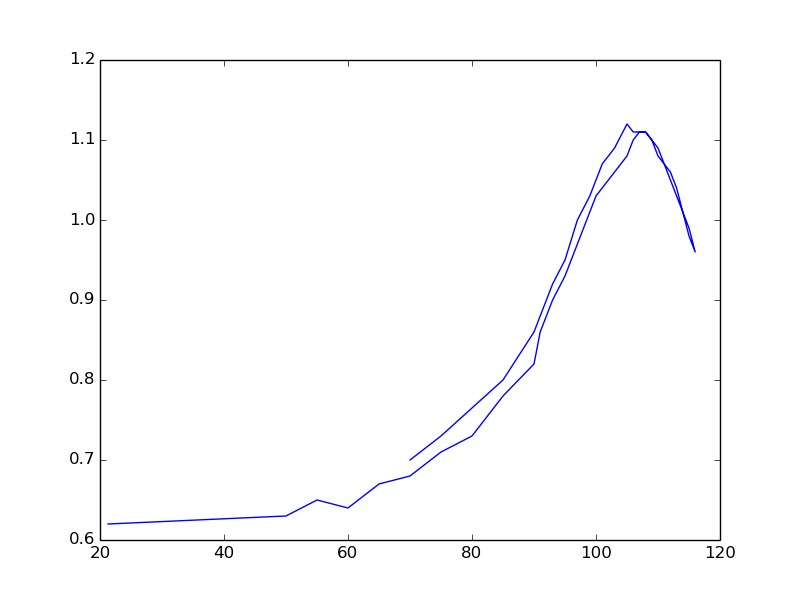
\includegraphics[scale = 0.5]{graphs/03table1.png}
\caption{Normal Transverse Zeeman Effect} 
\end{center}
\end{figure}
\end{center}


\section*{Results}

I'm too lazy to write my lab report.

\section*{Conclusion}

Conclusion

\end{document}

\end{document}
